\documentclass[12pt]{article}
\usepackage{flafter}
\usepackage{titlesec}
\usepackage[utf8]{inputenc}
\usepackage{hyperref}
\usepackage[mark=]{sectionbreak}
\usepackage{lipsum}
\usepackage{setspace}
\usepackage{titlesec}
\usepackage{graphicx}
\usepackage[T1]{fontenc}
\usepackage{titling}
\usepackage{geometry}
\setlength{\droptitle}{-2em}
\titleformat*{\section}{\LARGE\bfseries}

\hypersetup{
    colorlinks,
    citecolor=black,
    filecolor=black,
    linkcolor=black,
    urlcolor=black
}
\usepackage{tree-dvips}
\author{
  Khaled Abulawi\\
  \texttt{1531904}
  \and
  Ahmad J Alsoub\\
  \texttt{1837661}
  \and
  AL-Motasem Alamleh\\
  \texttt{1834683}
  \and
  \texttt{Supervised by, Dr.Aladdin Hussein Baarah 
  }
  \and 
  \texttt{ {\footnotesize Submitted in partial fulfillment of the requirements }
  }\and 
  \texttt{  {\footnotesize of B.Sc. Degree in Computer science}
  }}
\date{\today}
\title{5abini  \vspace{+1em}
\\ 
\includegraphics[width=0.1\textwidth]{logo.png}}
\raggedbottom
\begin{document}
\vbox{
    \centering
   
\includegraphics[width=0.2\textwidth]{Uni.JPG}
    \\  Software Engineering  
\\Faculty of Prince Al-Hussein Bin Abdallah II for Information Technology
\\The Hashemite University, Zarqa-Jordan
    \maketitle 
    \centering
}
\sectionbreak
\sectionbreak
\section*{Certificate}
It is hereby certified that the project titled <5abini>, Khaled Abulawi {1531904}, Ahmad Alsoub {1837661}, AL-Motasem Alamleh {1834683}, in partial fulfillment of the award of the Degree of Bachelor 
<Software Engineering> embodies original work done by them under my supervision\\ 
Project Supervisor: Aladdin Hussein Baarah \\ Department of Software Engineering.

\sectionbreak
\section*{Acknowledgment}
This project has given us an idea how companies may work and organize themselves. We had many hardships and challenges we had to go through, but the progress we made in a new language and workflow we never experienced made us proud. It's an experience we'll never forget.\\ \\ 
We would like to thank Dr. Alaa Ba'arah for his guidance and gearing our ideas in a better direction. Sharing some of his wisdom with us proved nothing but beneficial for us.\\ \\
We would also like to thank Dr. Bashar Al-Shboul and Dr.KHalid Al-Sarayreh for their assistance we needed them.\\
We wouldn't have made this app without your assistance, thank you all a lot for the support.
\sectionbreak
\section*{Abstract}
As people who lived a big major of their lives using Social media apps, and us being aware that newer generations will do the same, we, throughout our experiences, came to appreciate things we didn't consider in our earlier days, Privacy. \\
Nowdays, almost all social media apps focus on public interactions and people knowing who you are, we've seen success in this  trend of course, but we've also seen withdraw in actual human interactions or confrontation, because everyone knows who you are.\\  While discussing this subject, we came with the idea of an app that focuses on privacy, not because it hides your information, because it doesn't have it (the not so major ones at least). That's how 5abini was born.\sectionbreak
\


\tableofcontents
\sectionbreak







\section{Introduction}
\subsection{Background}
5abini as an app (that works on Android and IOS alike) focuses on privacy as a social media app. The usage of the application will be mostly from users and moderates, users will be able to:
\begin{enumerate}

\itemsep0em 
\item Browse posts by colleagues in the same facility
\item Comment on posts that interest them
\item Share interests, questions on the app directly to other people's feeds with posting a new post
\item Change apps looks if they choose to
\item Change facility if others interest them
\item Choose one of the default avatars
\item Write in both languages: Arabic and English
\end{enumerate}


\subsection{Problem statement}
Most social media platform are geared toward talking to people you already, or at least know they have something in common with you. There isn't a platform that allows you to share something that's not common between people and still get reactions and have some interactive experiences, as most there is a program as far as we can tell that links the posts you see geographically, there's features in some apps, but at that point the time line is so bloated that there's isn't roam for your niches.\\ 
\subsection{Objective}
5abini is an app that was built while focusing on privacy and intention to gather people with no social fear or anxiety. To  build an environment with confidence in confidentiality that allows you to share what you love, care about, ask questions and help people who do so. 5abini is geared into anonymous interactions, that will remove fear of social criticism and anxiety, as who you are will never be unknown. Make friends, get knowledge and share yours!



\section{literature review}
\subsection{Existing programs}
\subsubsection{Reddit}
Reddit allows users to comment and posts as "anonymous" but they generally collect user information and their UI isn't organized nor user friendly. You can easily be tracked down by other users since you post history is visible and on what "Thread (Hashtags)" you frequently use.
\subsubsection{Facebook}
As the biggest social media giant, we take it as granted that our information is safe, well kept, and untraceable, but because of the scale of information Facebook has, when a leak happens, 600 Million account information leak, we're built fundamentally different than Facebook and similar applications, this allows for a security that's hard to get, as you know closing the door is the better than setting traps and letting intruders come in.
\subsection{The effects on anxiety}
The findings suggest that the cognitive and behavioral processes that characterize socially anxious face-to-face interaction are also evident in online communication. Suggestions are made for the clinical implications of such findings.\cite{firstone}
\subsection{Privacy and Confidentiality}
Most of the social media sites have information that's required, like your birthday and email address. Identity thieves tend to gather their victims’s personal information from the information available on the social media sites. They argue there is a persistent confusion between these two concepts and that privacy is an important but neglected ethical concept within human services. Many identity thieves tend to hack their victims email accounts by simply using the personal information available on social media profile.\cite{Confidentiality}


\section{Requirement Elicitation}
In this sections, many argue requirement elicitation is the most important in creating software, we will be using approaches proposed by Alexander and Beus-Dukic.

\subsection{Identifying stakeholders} 
First of all, we have to identify the stakeholders (Clients), but as we (the participants) are the only Stakeholders, the elicitation we'll be conducted in methods that allow us to bring forth Ideas that will be as if they are requested by the client.
\subsection{Modeling the context (SCOPE)}
Before any step, we have to know what we're stepping into.
We had to understand and set the environment the Software and we will be working in. As the creators and developers, 
We had to always keep in mind that we'll be working inside the campus of Hashemite University, with the students and being our customers and users.
\subsection{Identifying scenarios and brainstorming}
We used hypothetical scenarios that users may go through, we asked ourselves what will they expect, how would they navigate, and what will they react to and focus on the most.
We'll see later on how this helped us build our user case.
\subsection{Analyzing priorities}
Priorities is a name we can easily replace "5abini" with, as it's already (as a software) geared into something very specific, we had no problems in seeing what should we focus on and what would our user base care about.
\section{Requirements}
\subsection{User requirements}
\begin{enumerate}
\itemsep0em 
\item User shall be able to sign up.
\item User shall be able to select an academy.
\item User Shall be able to select their major.
\item User shall be able to post.
\item User shall be able to delete their posts.
\item User shall be able to delete their comments.
\item User shall delete any comments on their posts.
\item User shall be able to report Posts.
\item User shall be able to report comments.
\item User shall be able to up-vote posts.
\item User shall be able to down-vote posts.
\item User shall be able to up-vote comments.
\item User shall be able to down-vote comments.
\item User shall be able to search for posts he's interested in, through Hash-tags or keywords.
\item User shall be named “Poster” when they post.
\item User shall be Assigned a “Name” that reflects their position in the post, the first time they interact.
\item User shall be able to track their activities.
\item User shall be able to track activities on their posts.
\item User shall be able to track activities on their comments.
\item User shall be able to review posts from other users.
\item User shall be able to sign out.

\end{enumerate}
\subsection{System Requirements}
\begin{enumerate}
\subsubsection*{Portability}
\item System shall run IOS, tablets and smart phones, and also emulators.
\subsubsection*{Security}
\item Database security is world class, provided by Google itself.
\item Flutter provides a secure data storage plugin for both the leading operating systems with the name of NSUserDefault for iOS and SharedPreferences for Android.
\subsubsection*{System and User Interaction}

\item User shall be able to sign up using their University number and Phone number.
\item System will check for any University number duplication upon sign up, if the system finds any, user shall be notified with a warning message.
\item User will have to confirm their identity with an OTP (One-Time-Password) that will be sent to confirm that they own the Phone number, and that it's correct.
\item User shall be able to assign a password that will agree with password requirements.
\item Passwords must use at least three of the four available character types: lowercase letters, uppercase letters, numbers, and symbols.
\item User shall be able to sign in with their Phone number and the OTP that will be sent.
\item User Shall be able to select the App’s theme after confirming their identity, the options will be “light-mode” and “dark-mode”.
\item User shall be able to comment on each post with a different name, unless it’s in their own posts, it will always be “Poster”, that will also show when they comment.
\item User that comment on a post will be given a name that reflects when they commented on the post (if they are the first to comment, their number will be @, second to comment will be @ Etc.)
\item User shall be able to report Posts by pressing the ellipsis button (three dots) on the post and selecting report. An interface will be shown, asking the user to select the reason for the report, and allowing the user to write his own personal reasoning and comments. The same procedure occurs with reporting comments.
\item User shall be notified with a “Pop-up” of activities related to their posts and comments.
\item User shall be able to Up-vote and Down-vote posts and comments by pressing Either the Up-vote button (arrow head pointing to the top) or Down-vote button (arrow head pointing to the bottom)
\item System shall only allow posts to last up to hours, user will have the option to select between and hours regarding his post availability.
\item User shall have an interface where they can see recent activities on their posts and comments that are still available.
\subsubsection*{System properties}
\item System should always be up, aside from maintenance

\item User's time-line shall be shown depending on the Major and academy they choose.
\item User shall be shown \# of posts, comments, upvotes, his most interacted post and recently available ones in the Account Interface.
\item An Admin will be assigned for human involvement if needed, giving them permission to delete others posts and comments.
\item System shall add posts, comment, delete, do other requests from 0.5 to 2 seconds maximum under heavy load.
\item System shall be able to handle 10000 thousand request at a time..
\end{enumerate}
\sectionbreak

\section{Models and Diagrams}
\subsection{USE CASE}
\vspace{-6em}
\begin{figure}[b]
\centerline{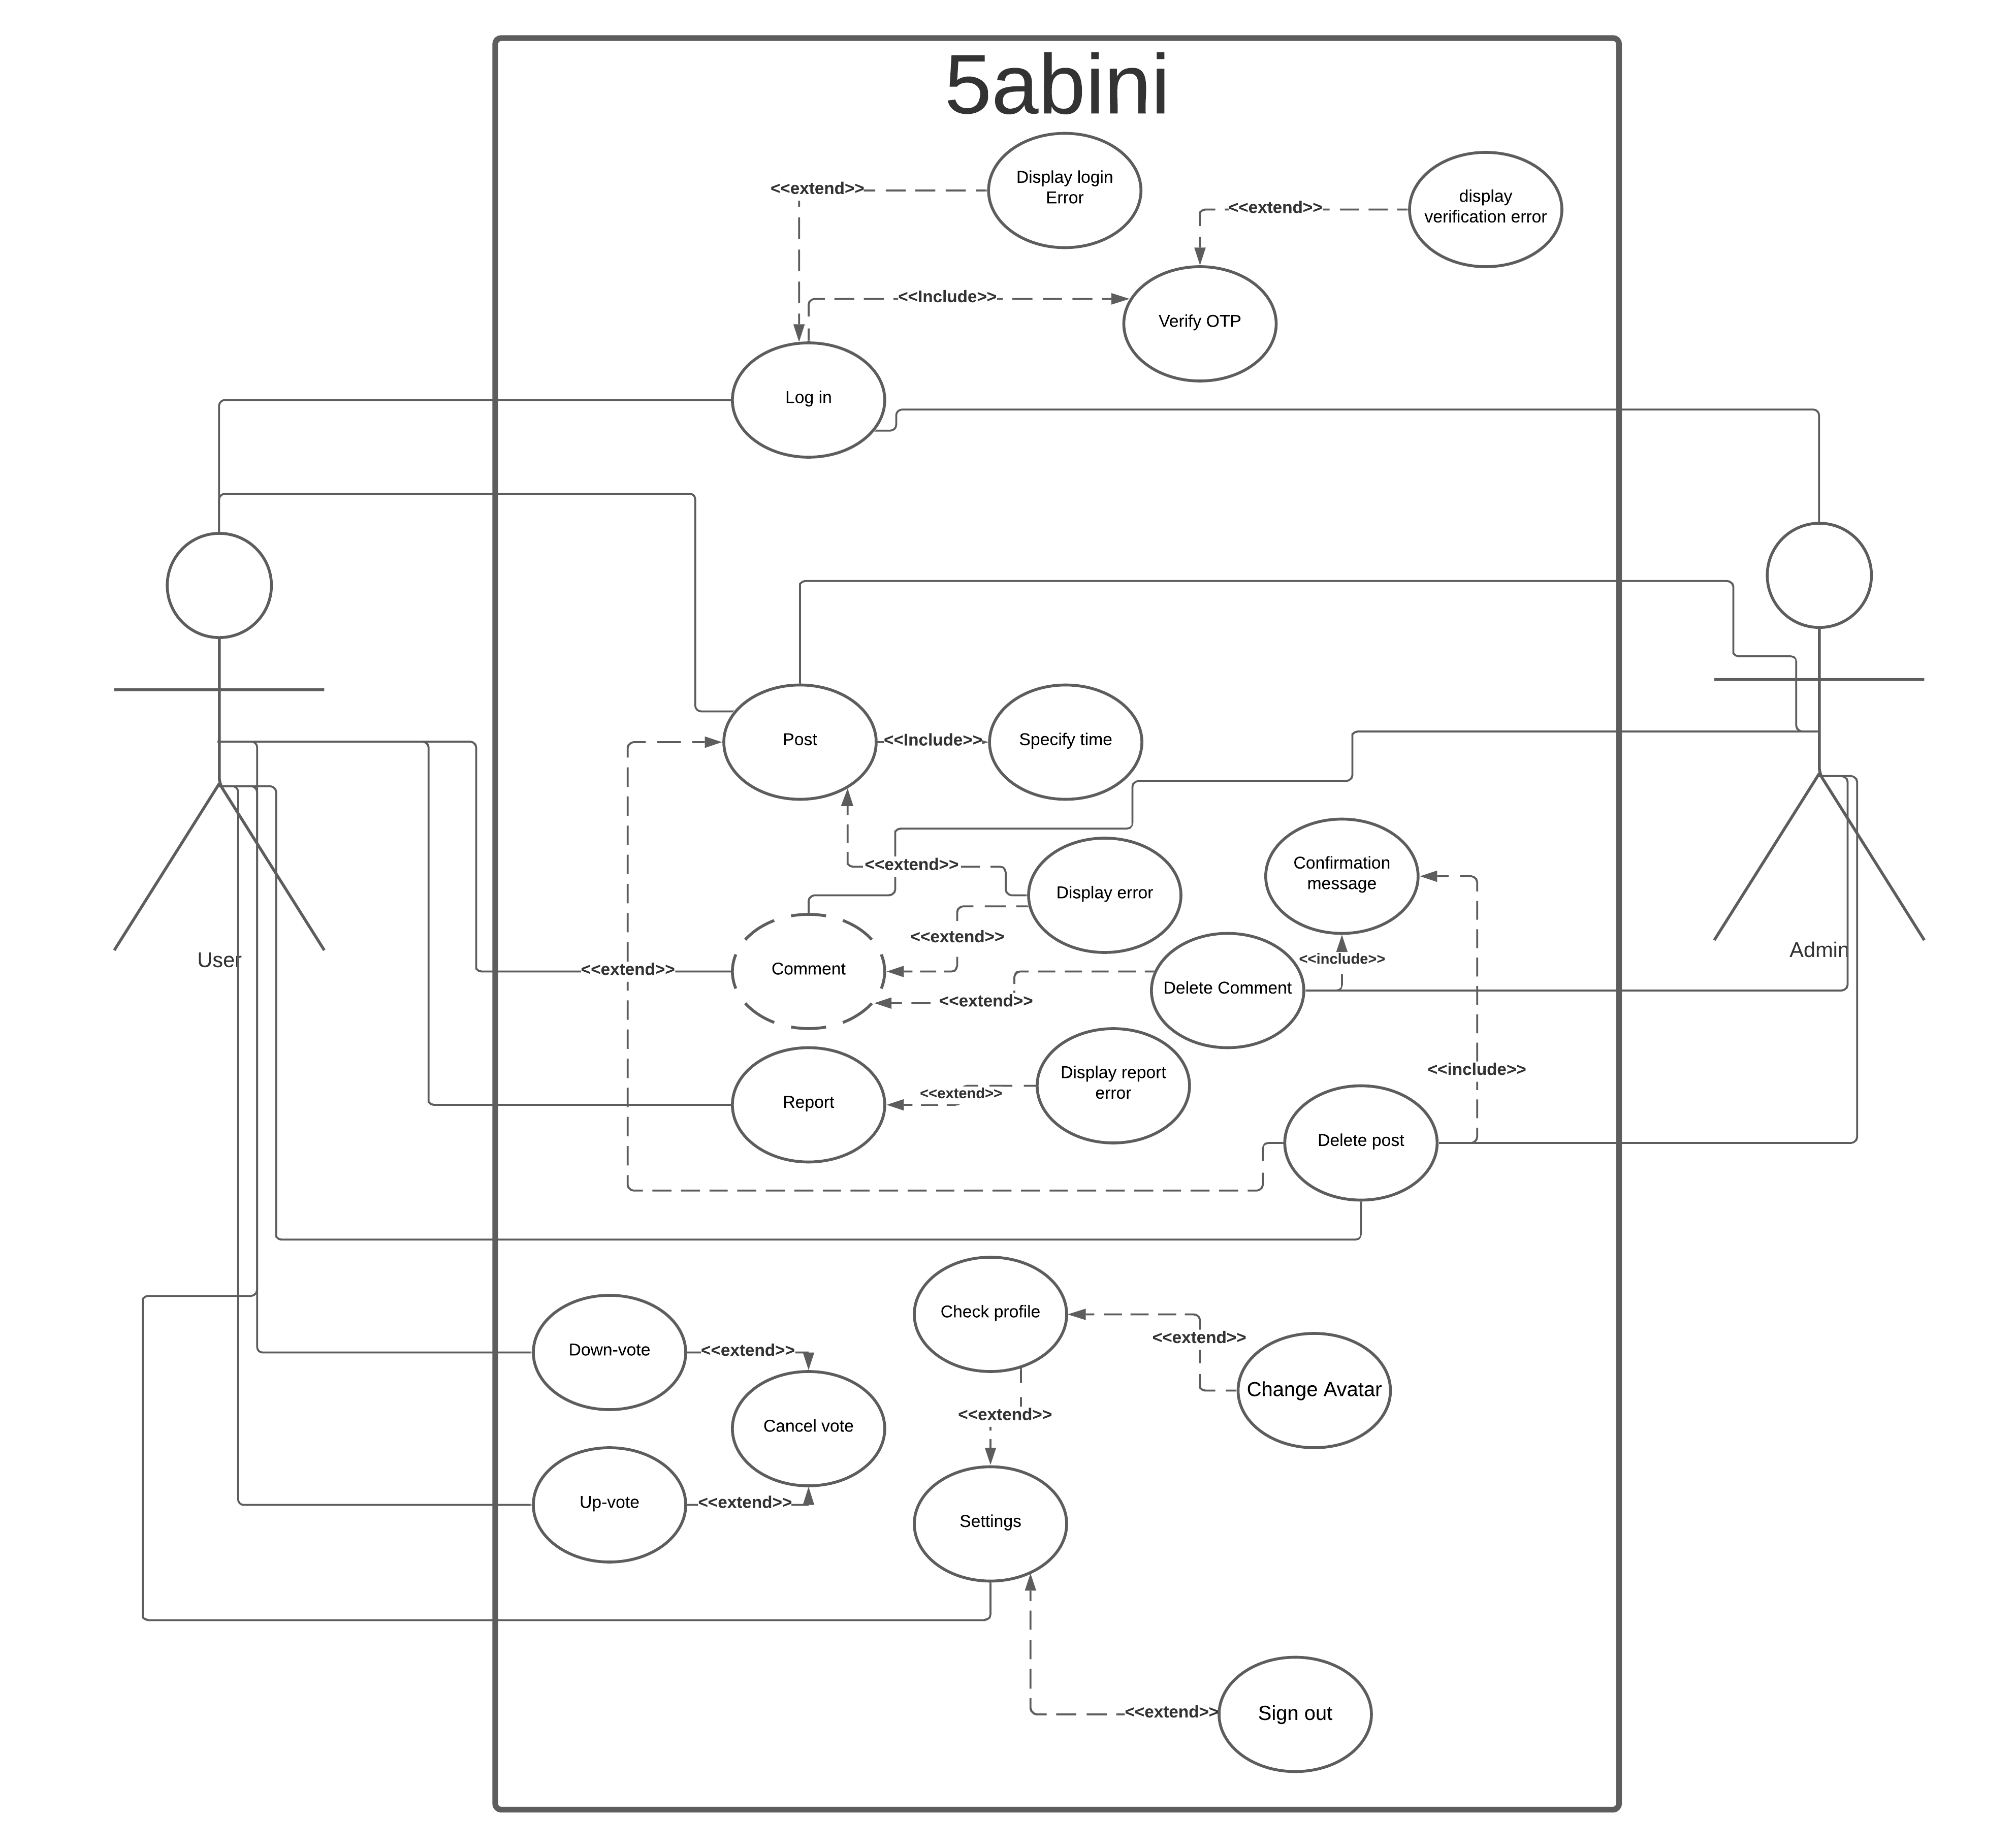
\includegraphics[width=1.4\textwidth]{./USECASE/5abiniUseCase.png}}
\vspace{-1em}
\caption{USE CASE}
\end{figure}
\twocolumn
\subsubsection{Use cases}
\subsubsection*{Log in}
\begin{enumerate}
\itemsep0em
\item Enter Phone number
\item Enter OTP
\item Click "Log in"
\end{enumerate}
\subsubsection*{Sign up}
\begin{enumerate}
\itemsep0em 
\item Enter University ID
\item Enter Phone number
\item Enter OTP
\item Click "Sign in"

\end{enumerate}
\subsubsection*{Post}
\begin{enumerate}
\itemsep0em 
\item Enter content
\item Set duration
\end{enumerate} 
\subsubsection*{Comment}
\begin{enumerate}
\itemsep0em 
\item Choose post
\item Press comment Icon
\item Enter content
\end{enumerate} 
\subsubsection*{Report}
\begin{enumerate}
\itemsep0em 
\item Click arrow to open list on post
\item Add report content
\item Click "Report"
\end{enumerate} 
\subsubsection*{Upvote-Downvote}
\begin{enumerate}
\itemsep0em 
\item Choose post
\item click Arrow-up to upvote, Arrow-down to downvote
\end{enumerate} 
\subsubsection*{Check Profile}
\begin{enumerate}
\itemsep0em 
\item Click on "Settings"
\item Click "Profile"
\end{enumerate} 
\subsubsection*{Delete account}
\begin{enumerate}
\itemsep0em 
\item Click on "Settings"
\item Click "Delete account"
\item Confirm Identity with OTP
\item Confirm delete
\end{enumerate} 
\subsubsection*{Change phone Number}
\begin{enumerate}
\itemsep0em 
\item Click on "Settings"
\item Click "Change phone"
\item Confirm Identity with OTP on old number
\item Enter new phone
\item Confirm Identity with OTP on new number
\end{enumerate}
\subsubsection*{Change location}
\begin{enumerate}
\itemsep0em 
\item Click on "Settings"
\item Click "Location"
\item Choose "A Facility
\item Click "Change"
\end{enumerate}
\subsubsection*{Sign out}
\begin{enumerate}
\itemsep0em 
\item Click on "Settings"
\item Click on "Sign out"
\end{enumerate}
\onecolumn
\sectionbreak
 \subsection{ER Diagram}
\begin{figure}[h!]
\centerline{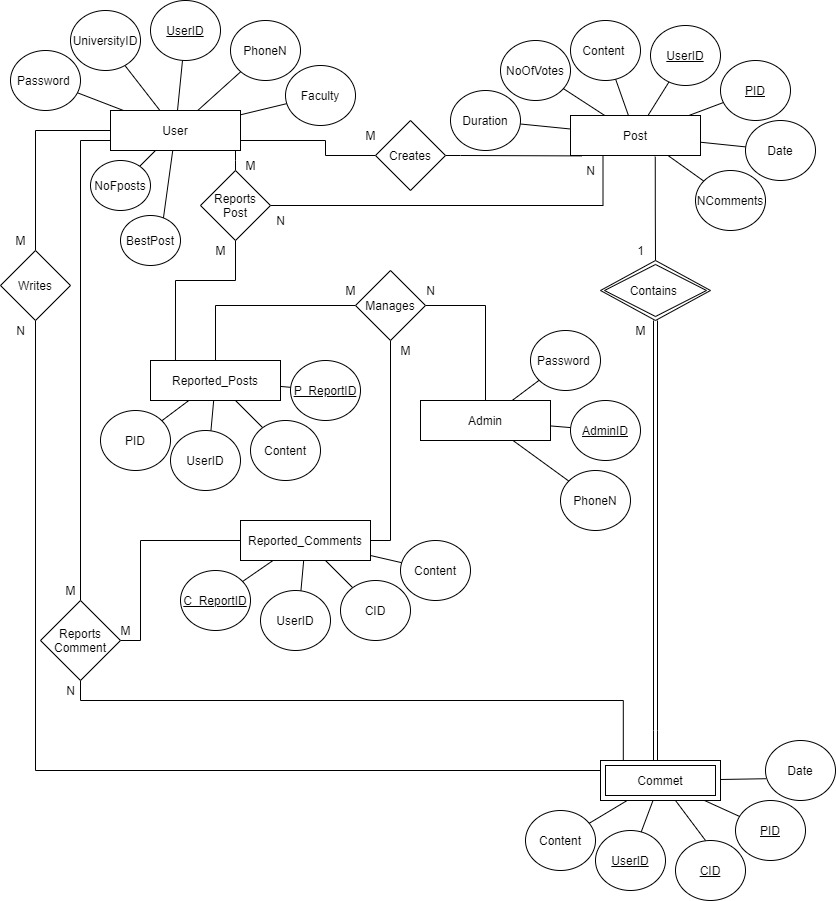
\includegraphics[width=0.95\textwidth]{./ERDiagram/ERDiagram.JPG}}
  \caption{ER Diagram}
\end{figure}

\vspace{-1em}
\subsection{Sequence Diagrams}
\subsubsection{Sign-up}
\begin{figure}[h!]
\centerline{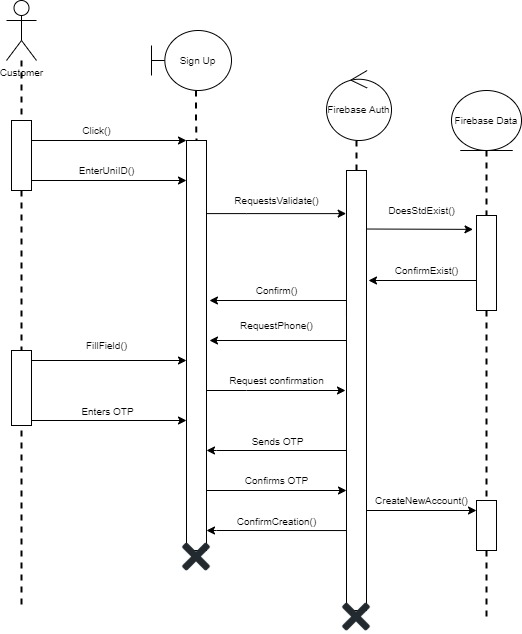
\includegraphics[width=0.85\textwidth]{./SequenceDiagram/SequenceDiagram.JPG}}
  \caption{Sign-up sequence}
\end{figure}
\clearpage
\subsubsection{Post}
\begin{figure}[h!]
\centerline{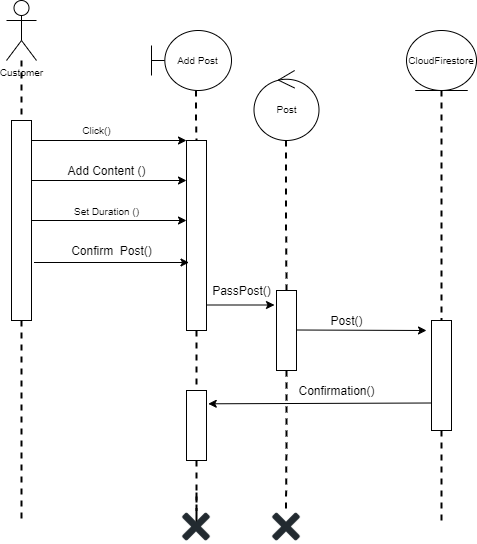
\includegraphics[width=0.85\textwidth]{./SequenceDiagram/SequenceDiagram2.PNG}}
  \caption{Sign-up sequence}
\end{figure}

\sectionbreak
\vspace{+6em}
\subsubsection{Class Diagram}
\vspace{-1.4em}
\begin{figure}[h!]
\centerline{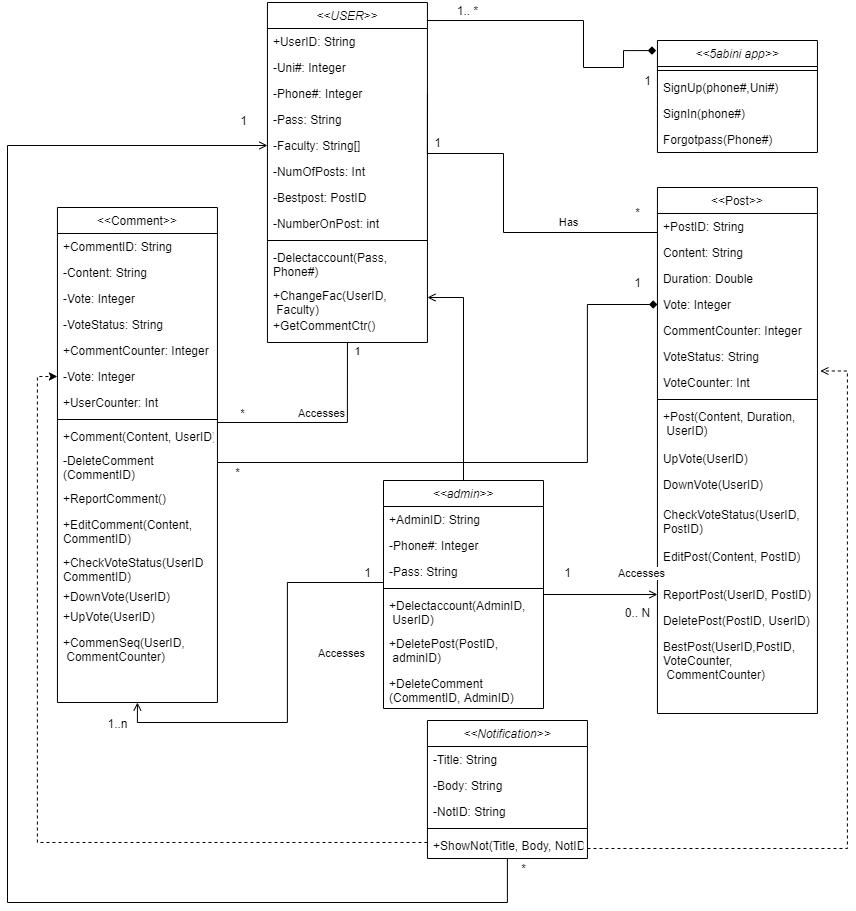
\includegraphics[width=1.1\textwidth]{./ClassDiagram/ClassDiagram.PNG}}
  \caption{Class Diagrams}
\end{figure}
\clearpage
\subsection{Software Architecture}
\centerline{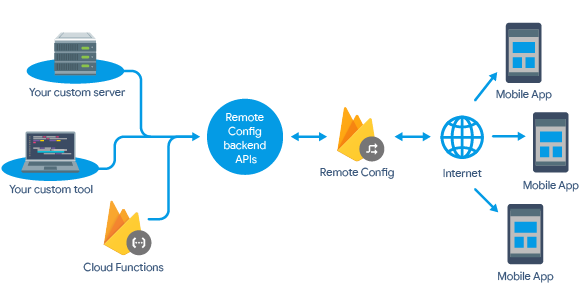
\includegraphics[width=1.1\textwidth]{./SoftwareArch/SoftwareArch.PNG}}
\section{Software Implementation and Testing}
\subsection{Tools}
\begin{itemize}
  \item  LaTeX (Academic document preparation tool) 
  \item  Android Studio (for Coding)
  \item  Github (Documentation and Code sharing)
  \item  Firebase (Used to maintain fully functional cloud-based database that's encrypted by google)
  \item  JSON
  \item  Lucid Chard (Diagrams and models)
  \item  Draw.io (Diagrams and models)
  \item  Firebase Authentication (API's that are used for user Authentication) 
\subsection{Languages}
\item Flutter
\item Java.js

\end{itemize}
\bibliographystyle{plain}
\bibliography{Citation}
\end{document}